% Fig. 3.26 -- the i-th order statistic Y_i splits the support into two
%   stretches: i-1 of the sample lie to its left, n-i to its right.
% Source: mathstatch3.tex lines 5324-5338.  Manuscript geometry kept: the
%   same number line as Fig. 3.24, a divider at x = 5 named y_i, the counts
%   above the line at x = 2.5 and x = 7.5, and two dashed arcs under the line
%   spanning 0 to 5 and 5 to 9.95, labelled with the probability that one
%   sample value falls in that stretch.
%
% Third of the series 3.24-3.27; coordinates, divider height, arc depth and
% type size are those of order-stat-min.tex, and the four departures from the
% manuscript picture recorded there apply here unchanged (counts left as bare
% mathematics, y_i carried at the top of the divider, arcs drawn as cubics of
% sag 0.40, F_{\sssig X} written F_X).  The third of them bites hardest in
% this figure: the manuscript leaves both bend angles at 30 degrees over
% spans of 5 and 4.95, which would sink both arcs to 0.62 units, half again
% as deep as the arcs of the three neighbouring figures.
%
% \DeclareMathSizes{10}{10}{9}{8} raises the math script sizes from the
% default 7pt/5pt.  Native width 249.343pt (drawing range 8.63cm, inside the
% 9.0cm cap of spec 1.3).  A mark of S pt shows at
% S x 0.99626 x <display width> / 249.343 px, so in a topic-figure--wide at the
% 350px phone width
%     10pt text 13.98px, 9pt scripts 12.59px
% and at the 620px desktop width 24.77 / 22.30px.  The smallest marks in the
% picture are the X of F_X and the i of y_i, both at script size.
\documentclass[tikz,border=2pt]{standalone}
\usepackage{amsmath}
\usepackage{amssymb}
\usepackage{xcolor}
\usetikzlibrary{arrows.meta}
\DeclareMathSizes{10}{10}{9}{8}

\definecolor{journalink}{HTML}{1F1C18}
\definecolor{journalmuted}{HTML}{8A7F72}
\definecolor{journalaccent}{HTML}{9C2D2D}

\begin{document}
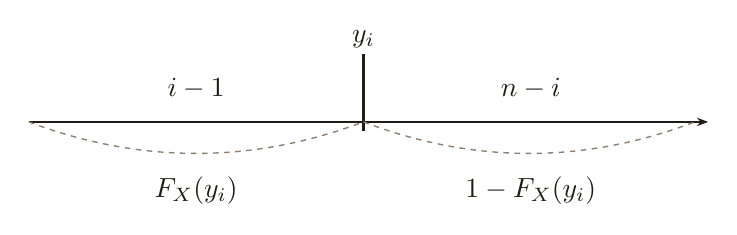
\begin{tikzpicture}[
  x=0.85cm,
  y=1cm,
  every node/.style={font=\normalsize, journalink, inner sep=1pt},
  axis/.style={journalink, line width=0.8pt, -{Stealth[length=4pt]}},
  divider/.style={journalink, line width=0.8pt},
  arc/.style={journalmuted, line width=0.5pt, dash pattern=on 2pt off 2pt}
]
  % ---- the number line -------------------------------------------------
  \draw[axis] (0,0) -- (10.15,0);

  % ---- the cut at y_i --------------------------------------------------
  \draw[divider] (5,-0.12) -- (5,0.86);
  \node[anchor=south] at (5,0.90) {$y_i$};

  % ---- how many of the sample lie in each stretch ----------------------
  \node at (2.5,0.43) {$i-1$};
  \node at (7.5,0.43) {$n-i$};

  % ---- the probability of each stretch ---------------------------------
  \draw[arc] (0,0) .. controls (1.6667,-0.5333) and (3.3333,-0.5333) .. (5,0);
  \draw[arc] (5,0) .. controls (6.65,-0.5333) and (8.3,-0.5333) .. (9.95,0);
  \node[anchor=north] at (2.5,-0.65) {$F_X(y_i)$};
  \node[anchor=north] at (7.5,-0.65) {$1-F_X(y_i)$};
\end{tikzpicture}
\end{document}
